\hsection{Software}%
\label{sec:software}%
\FloatBarrier%
%
\begin{figure}%
\centering%
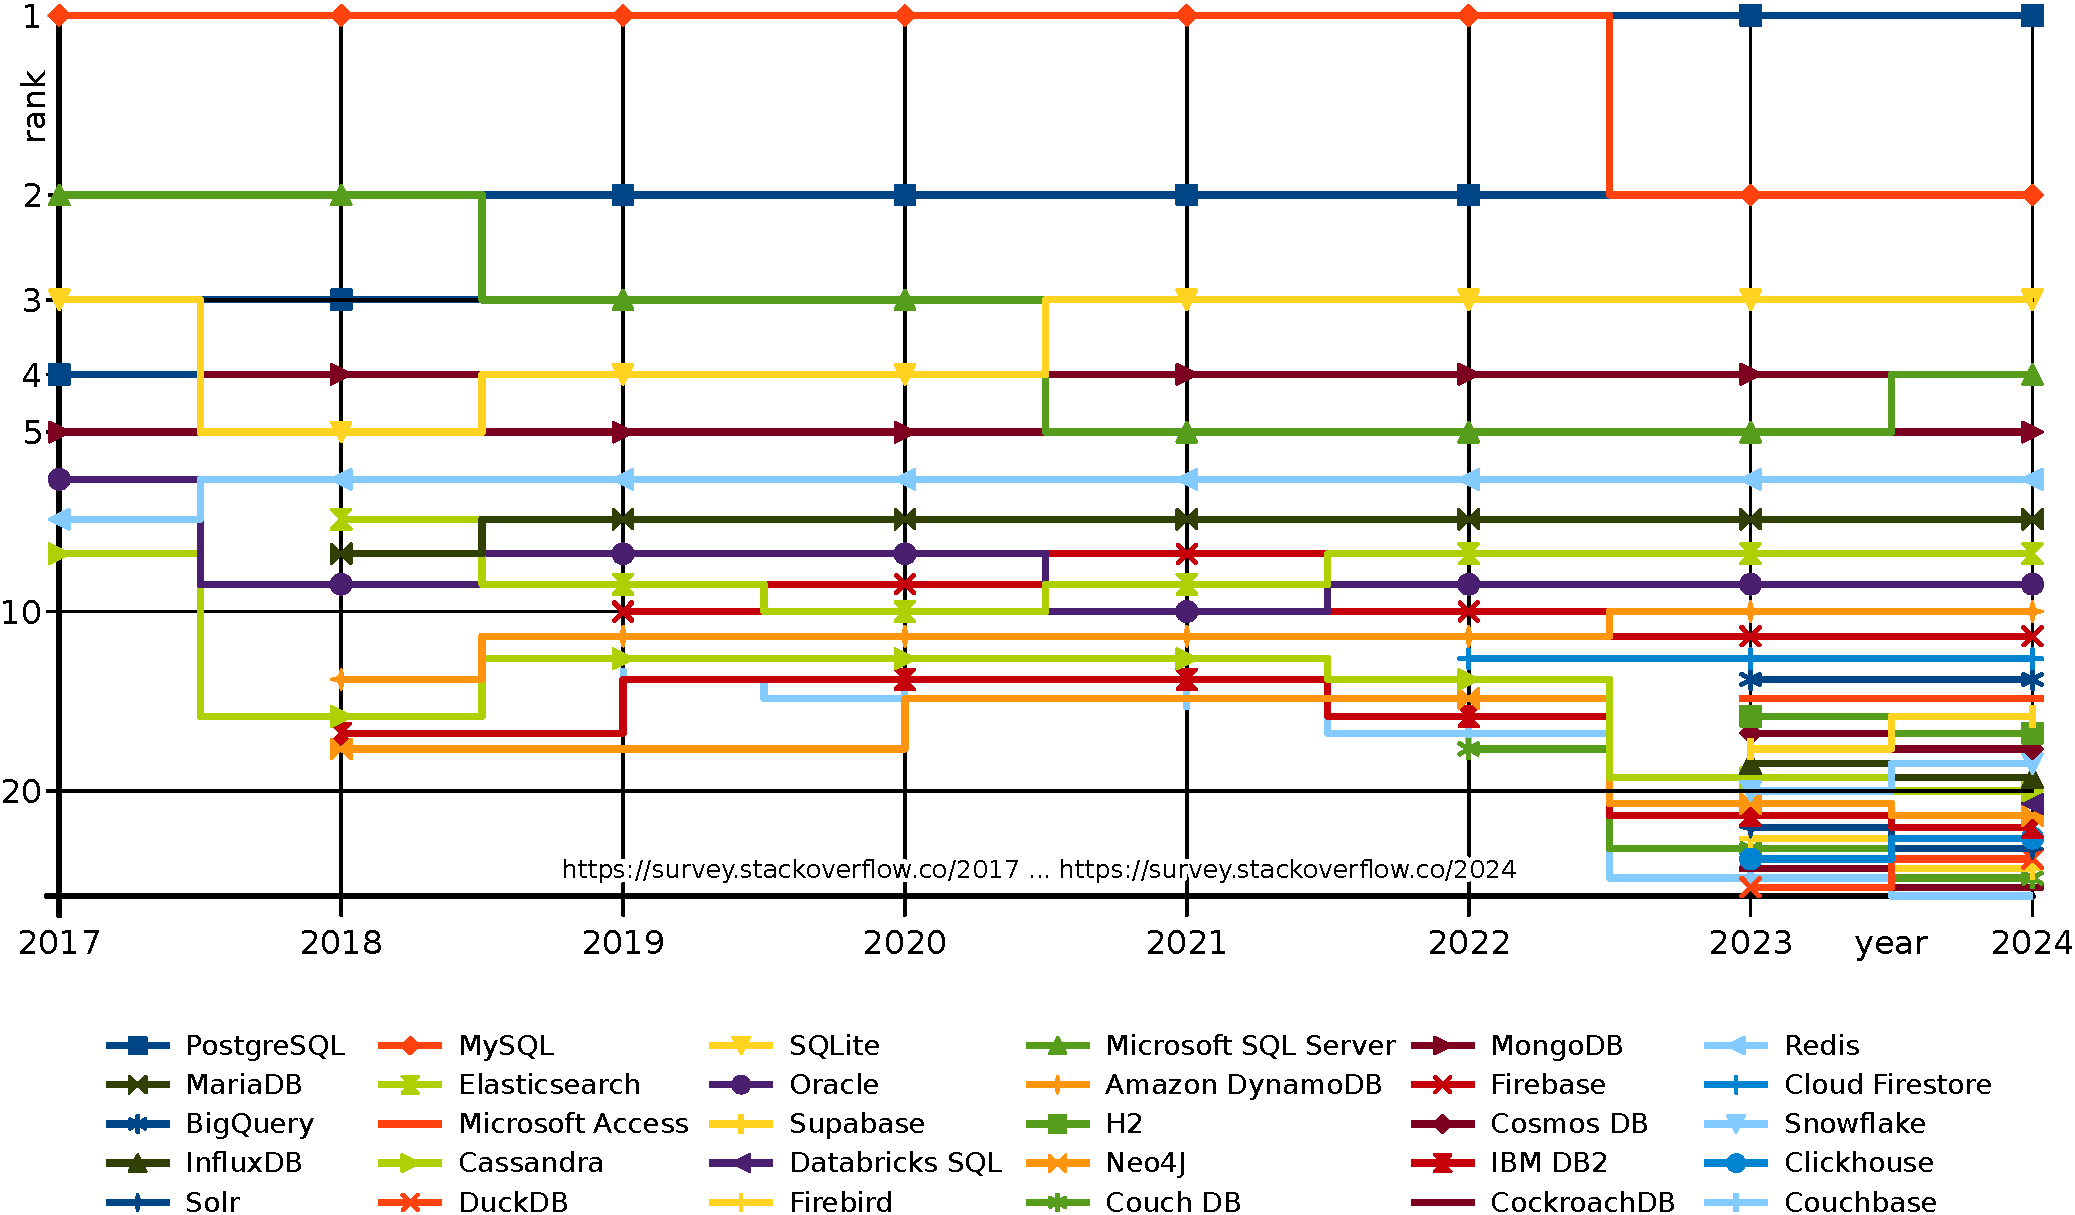
\includegraphics[width=0.99\linewidth]{\currentDir/soDevSurv}%
\caption{A chart of a selection of the \pglspl{dbms} with which developers have worked, according to the StackOverflow Developer Surveys from 2017 to 2024~\cite{SE:SO:2024DS}. %
Not all of them are relational \pglspl{dbms}.}%
\label{fig:soDevSurv}%
\end{figure}%
%
A wide range of \pglspl{dbms} for \pglspl{rdb} exist.
The \begin{noglslink}\citetitle{RS2025DERORD}\end{noglslink}~\cite{RS2025DERORD} lists 166 products.
The \citetitle{SE:SO:2024DS} asked the opinions of developers on 35 systems~\cite{SE:SO:2024DS}.
A selection of the mentioned systems in these yearly surveys since 2017 is illustrated in \cref{fig:soDevSurv}.
A few of these popular \pglspl{dbms} were already mentioned in our history section.
We can distinguish two types of \db\ products:%
\begin{itemize}%
%
\item \glsreset{OSS}\Pgls{OSS} is software whose source code is made availabe for free, usually through the internet.
Such software is often maintained by groups of volunteers, sometimes with financial support of enterprises or governmental grants.
The software does not cost money.
Open source projects are often hosted on collaborative platforms like \github\ and manage the evolution of their code via \pglspl{VCS} like \git.
According to \citeauthor{HNZ2024TVOOSS} the value of \pgls{OSS} exceeds eight trillion dollars in~\citeyear{HNZ2024TVOOSS}~\cite{HNZ2024TVOOSS}.
%
\item Proprietary / commercial software is usually closed-source and developed by an enterprise which sells it as product.
These products are either sold on a per-version basis or via maintenance contracts.
The enterprises often offer good service and advanced support, however it is usually not easy to change vendors and future pricing developments are hard to predict.%
%
\end{itemize}%
%
We here will discuss a small selection of products from either family, which, however, must remain brief and incomplete.%
%
\hsection{Open Source Relational Database Management Systems}%%
%
\begin{figure}%
\centering%
%
\subfloat[][%
The \mariadb\ logo.%
]{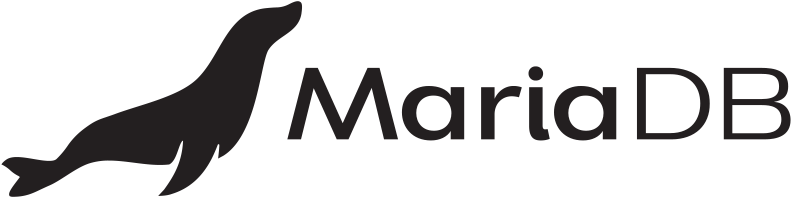
\includegraphics[height=1.75cm]{\currentDir/mariadbLogo}}%
%
\floatSep%
%
\subfloat[][%
The \postgresql\ logo.%
]{
\includegraphics[height=1.75cm]{\currentDir/postgresqlLogo}}%
%
\floatSep%
%
\subfloat[][%
The \sqlite\ logo.%
]{
\includegraphics[height=1.75cm]{\currentDir/sqliteLogo}}%
%
\floatRowSep%
%
\subfloat[][%
The \libreoffice\ logo.%
]{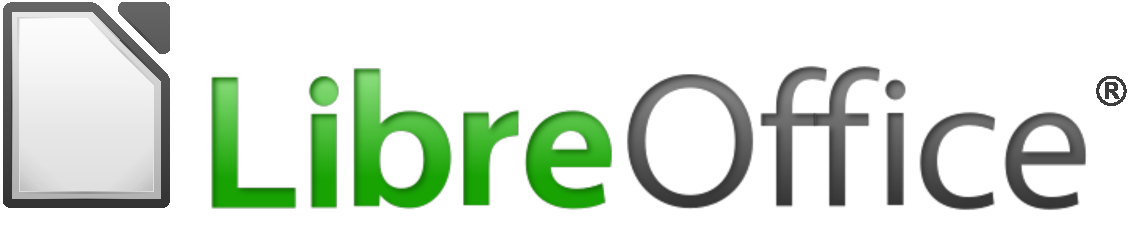
\includegraphics[height=1.35cm]{\currentDir/libreofficeLogo}}%
%
\caption{The logos of several important \pglspl{OSS} / \pglspl{dbms}.}%
\label{fig:ossDBlogos}%
%
\end{figure}%
%
A very big chunk of the \pglspl{rdb} is managed by open source \pglspl{dbms}.
These systems do not cost money and their source code is readily available in the internet.
Large communities exist around them that can offer all kinds of advise.
This makes them very attractive for developers and users.
Several of these systems are around since the 1990s.
In the early 2000s, they took off and began being used in more and more applications and systems~\cite{P2004OSDMITM}.
By now, they are mature and well-tested products~\cite{C20245YOQ}.
\Cref{fig:ossDBlogos} shows some of their logos.

\mysql\ is such an open source \pgls{dbms} for \pglspl{rdb}~\cite{WAM2002MRMDFTS,TA2024DDAMWPAM,BT2021HPM,RGS2021BTOTONAMDFPC,D2015LMAM}.
It was originally developed by Michael Widenius and David Axmark at the Swedish company \mysql~AB and released in 1996~\cite{C20245YOQ}.
It soon gained widespread use as part of the \lampStack, i.e., a system setup for web applications based on the \linux\ \pgls{OS}, the Apache webserver, the \mysql\ database, and the \pgls{server}-side scripting language~PHP~\cite{C2022HAFTLS,H2020ULU2E}.
Probably as the result of this, it ranked first in the Stack Overflow Developer Surveys in the years 2017 to 2022~\cite{SE:SO:2024DS}.
In the recent survey~\cite{PMPVEPWGSMB2025ATAODMSTTHOOSP} of the code of 371~\pgls{Java} open source projects on \github, \mysql\ was found to be the most-used relational \pgls{dbms}.
\mysql~AB was acquired by Sun Microsystems in 2008, which in turn was acquired by Oracle in 2010~\cite{C20245YOQ}.
\mysql\ staied open source.

After the acquisition by Oracle, some of the original developers of \mysql, including Michael Widenius, created a fork of \mysql:~\mariadb~\cite{R2014MM,B2019LTMEELFFSAA,D2015LMAM,AA2018QAWMV1ITSQ,AA2018QAWMV2IDQ}.
They promise that \mariadb\ will stay open source forever.
In \cite{PMPVEPWGSMB2025ATAODMSTTHOOSP}, \mariadb\ was already the fifth most popular relational~\pgls{dbms}.

\postgresql~\cite{TA2024DDAMWPAM,FP2023LP,OH2017PUAR,B2024PELUYDW} is an object-relational \pgls{dbms}, meaning that it supports concepts from \pgls{OOP}, such as inheritance relationships between tables.
It also supports many additional types like \pgls{JSON} objects and geometric types.
\postgresql\ emerged from the POSTGRES project, the successor of the INGRES project at the University of Berkeley in California~\cite{C20245YOQ}.
It may be the most fully-featured of the existing open source \pgls{SQL} \pglspl{dbs}
In the \citetitle{SE:SO:2024DS}, it was the most popular \pgls{dbms}~\cite{SE:SO:2024DS} and in the open source code survey~\cite{PMPVEPWGSMB2025ATAODMSTTHOOSP}, it ranked second.

The \pgls{SQL} \pgls{db} with the widest distribution is \sqlite~\cite{WB2019RHSOOS,GPBHKP2022SPPAF,C20245YOQ,HWACIS:HO2023WKUOS}.
It breaks with the common approach to offer access to the \pgls{db} follwing a \gls{clientServerArchitecture}.
Instead, it is directly loaded as a library in the process that uses.
Today, it is installed on nearly every smartphone, computer, web browser, television, and automobile~\cite{WB2019RHSOOS,GPBHKP2022SPPAF,C20245YOQ}.
It was first released in 2000 and its core designer Richard Hipp received the SIGMOD Systems Award in 2017~\cite{C20245YOQ}.

The concept of \pglspl{dbms} that can work on stand-alone files is also implemented in the open source office suite \libreoffice~\cite{DF2024LTDF,GL2012LTSOOSSCBAFACSOL,S2022L7PFEUU}: \libreofficeBase~\cite{FNFHWSKLSSGLFRSRPLJG2022BG7R1BOL7C,S2022L7PFEUU}.
\libreofficeBase\ is more than a \pgls{dbms} working on single file.
Instead, it offers a powerful user interface that can also connect to databases such as \mysql, \mariadb\ and \postgresql.
The user interface allows you to conveniently design tables, views, queries, forms, and reports for the \pglspl{db} it connects to.
\libreofficeBase\ is a free alternative to the commercial product \microsoftAccess~\cite{SSI2023MA2BTA,B2020HOMA2,UC2021AFD}, which offers a similar functionality.

Many of the examples used in this book will be implemented based on \postgresql\ and we will also play around with \libreofficeBase.%
%
\endhsection%
%
\hsection{Commercial Relational Database Management Systems}%
%
There are many powerful commercial \pglspl{dbms}.
Different from the open source solutions, they do cost money and their source code is closed, i.e., the user cannot access it and only has an installer and program binaries to work with.

As already discussed, the first commercial \pgls{SQL}-based product was the \oracleDB~\cite{C20245YOQ,O2007OTHTMIMIOHWCFTPWMIH}.
This product is still one of the most successful and widely used commercial \pglspl{db} with many advanced features~\cite{BBDDSY2011ADOODM,KK2021EODATASFHPAP}.
In June~2025, it ranked first as most popular \pgls{dbms} in~\cite{RS2025DERORD} and it was the fourth most popular \pgls{dbms} in \cite{PMPVEPWGSMB2025ATAODMSTTHOOSP}.
How to migrate an \oracleDB\ to \postgresql\ is discussed in~\cite{KO2023DMFOTP}.

The third-ranking \pgls{dbms} in~\cite{RS2025DERORD} was the \microsoftSqlServer~\cite{P2020MSS2ABG,A2024TSAFMSS2,W2018MSSDB}.
This \pgls{dbms} dates its roots back to 1988, when Microsoft, Ashton-Tate, and Sybase collaborated to create a variant of Sybase \sql\ Server for the \pgls{OS} IBM~OS/2~\cite{W2018MSSDB:TEOMSS}.
The first version of this new \db\ server was released in 1989.
Later versions were released for \microsoftWindows~NT.
Today, like \oracleDB, it also runs on \linux.
With \microsoftAccess~\cite{LF2022MOSBSO2AM3}, Microsoft also offers a \pgls{dbms} mainly used on single computers by single users.
It is an incredibly useful and convenient tool, which combines the features of a \pgls{rdb} with advanced form design and reporting features~\cite{SSI2023MA2BTA,B2020HOMA2,UC2021AFD,MM2014RDAMA}.
This system is probably the role model after which \libreofficeBase\ was shaped.
Most things that can be done with \libreofficeBase\ that we will explore can just as well be done with \microsoftAccess, in many cases even more conveniently~(but \libreofficeBase\ is free\dots).

IBM's \ibmDB~\cite{CWDS2007UDLVWE,BBBCCDMMP2016SPTAFOIDFI} is another early relational \dbms~\cite{HS2013THAGOID}.
It emerged as a software for powerful mainframe computers that IBM manufactured themselves.
Mainframes are very powerful central computers, often used by large organisations and businesses.
While Oracle focussed on providing \pglspl{db} for normal computers, IBM focussed on powerful central \pglspl{server}.
By 1989, half of all mainframe customers had \ibmDB\ installed~\cite{HS2013THAGOID}.
\ibmDB\ still ranked sixth in the~\begin{noglslink}\citetitle{RS2025DERORD}\end{noglslink}~\cite{RS2025DERORD} and 23rd in the \citetitle{SE:SO:2024DS}~\cite{SE:SO:2024DS}.%
%
\endhsection%

Of course, we here can only give a very brief and very incomplete overview on the different open source and commerical relational \pglspl{dbms} on the market.
The vast number of such systems and the fact that they are core cash cows for huge companies such as Microsoft, Oracle, and IBM underline the importance of this field.
In our journey, we will use the free \postgresql\ as platform to experiment with \pglspl{db}, which makes sense because it is the top-ranking \pglspl{dbms} in~\cite{SE:SO:2024DS}, ranks fourth in~\cite{RS2025DERORD}, and is, well, free.%
%
\endhsection%
%
